\documentclass{ximera}

\author{Anna Davis} \title{MTH 140 Homework 4} 

\begin{document}

\begin{abstract}

\end{abstract}
\maketitle
% \textit{Certificate due: 2/22/2021 at 11:59 p.m.}
 
 \begin{problem}\label{prob:140hom4prob1}
A fair coin is tossed Twice.  
\begin{enumerate}
    \item Fill out the following table to help you determine probabilities of obtaining various outcomes.
    
\begin{center}
\begin{tabular}{|c|c|c|}
 \hline
 &&   \\
 & H& T  \\
 &&   \\
  \hline
  &&\\
 H&$\answer{HH}$&$\answer{HT}$ \\
  && \\
 \hline
  &&\\
 T&$\answer{TH}$&$\answer{TT}$ \\
  && \\
 \hline
 \end{tabular}
\end{center}    
\item Probability of getting one tail: $\answer{0.5}$

\item Probability of getting two heads: $\answer{\frac{1}{4}}$
\item Probability of getting three tails: $\answer{0}$
\end{enumerate}
\end{problem}

\begin{problem}\label{prob:140hom4prob2}
A conference caterer determines the probabilities of a workshop attendee drinking 0, 1, 2, 3, or 4 cups of coffee during the workshop.  Probabilities are listed in the table below.  Use this information to complete the table and answer the questions.

\begin{center}
\begin{tabular}{|c|c|c|}
 \hline
 &&    \\
 Cups of Coffee ($x$) & $P(x)$& $xP(x)$  \\
 &&   \\
  \hline
  &&  \\
 \quad$0$\quad&$0.05$&$\answer{0}$ \\
  && \\
 \hline
  && \\
 \quad $1$&$0.45$&$\answer{0.45}$  \\
  && \\
 \hline
  && \\
  \quad $2$&$0.35$& $\answer{0.7}$  \\
  && \\
 \hline
  & &\\
 \quad $3$& $0.12$&$\answer{0.36}$  \\
  &&\\
 \hline
  & &\\
 \quad $4$&$0.03$ & $\answer{0.12}$ \\
  &&\\
 \hline
\end{tabular}
\end{center}

\begin{enumerate}
    \item Expected value: $\mu=\answer{1.63}$
    \item What percentage of attendees is expected to drink one cup of coffee?
$$\answer{45}\%$$
\item What percentage of attendees is expected to drink 2 or more cups?
$$\answer{50}\%$$
    \item Which of the following is the most correct practical interpretation of the expected value $\mu$?
    \begin{multipleChoice}  
\choice{Every workshop attendee is expected to drink approximately one and a half cups of coffee.}  
\choice{If a workshop has 5 attendees, then approximately $8$ cups of coffee will be consumed.} \choice[correct]{If the workshop has 120 attendees, then approximately $200$ cups of coffee will be consumed.}  
\choice{This expected value is not an integer.  It must be rounded to the nearest integer for it to be meaningful.} 
\end{multipleChoice}
\end{enumerate}

\end{problem}


\begin{problem}\label{prob:140hom4prob3}
The diagram below shows two spinners.  (The arrow spins and points to one of three numbers.)  Two spinners are spun and the values are added together.  Let $X$ be the sum of the values.  

\begin{image}
   
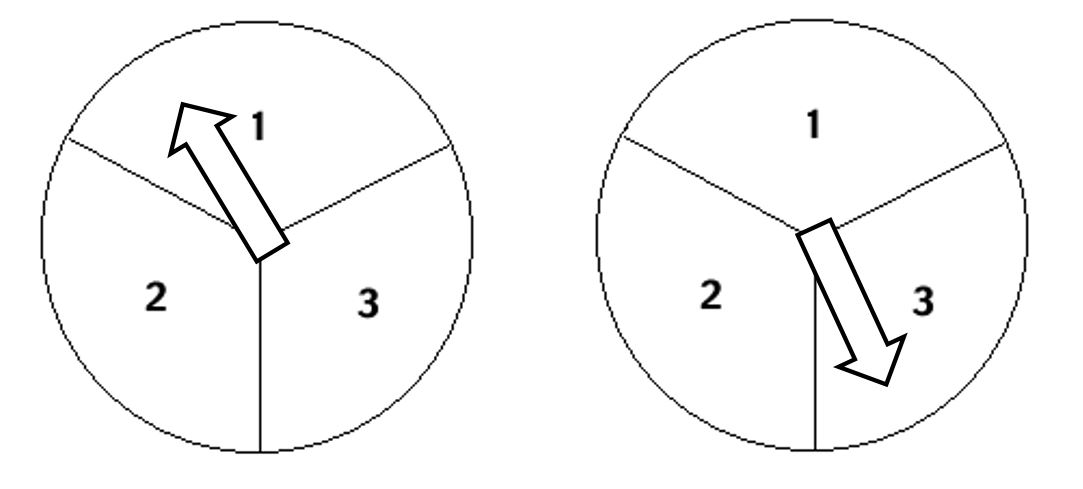
\includegraphics[height=1in]{140H4pic1.jpg}~
 
\end{image}



\begin{enumerate}
    \item Fill out the following table to help you determine probabilities of obtaining various sums.
    
\begin{center}
\begin{tabular}{|c|c|c|c|}
 \hline
 && &   \\
 & $1$& $2$ &$3$ \\
 && &   \\
  \hline
  && & \\
 $1$&$\answer{2}$&$\answer{3}$&$\answer{4}$ \\
  &&& \\
 \hline
  &&& \\
 $2$&$\answer{3}$&$\answer{4}$ &$\answer{5}$ \\
  &&& \\
 \hline
  &&& \\
  $3$&$\answer{4}$&$\answer{5}$  &$\answer{6}$ \\
  &&& \\
 \hline
 \end{tabular}
\end{center}    
    
    
\item Find the probabilities. Please use EXACT values, not decimal approximations. (E.g. use fractions.)
$$P(1)=\answer{0}$$ $$P(2)=\answer[tolerance=0.01]{\frac{1}{9}}$$ $$P(4)=\answer[tolerance=0.01]{\frac{1}{3}}$$ $$P(x<10)=\answer{1}$$ $$P(x\leq 4)=\answer[tolerance=0.01]{\frac{2}{3}}$$


\item Fill out the table provided below and find the expected value $(\mu)$ and the standard deviation $(\sigma)$.  

\begin{center}
\begin{tabular}{|c|c|c|c|}
 \hline
 && &   \\
 Sum of Values ($x$) & $P(x)$& $xP(x)$ &$(x-\mu)^2P(x)$ \\
 && &   \\
  \hline
  && & \\
 \quad$2$\quad&$\answer[tolerance=0.01]{\frac{1}{9}}$&$\answer[tolerance=0.01]{\frac{2}{9}}$&$\answer[tolerance=0.01]{\frac{4}{9}}$ \\
  &&& \\
 \hline
  &&& \\
 \quad $3$&$\answer[tolerance=0.01]{\frac{2}{9}}$&$\answer[tolerance=0.01]{\frac{2}{3}}$ & $\answer[tolerance=0.01]{\frac{2}{9}}$ \\
  &&& \\
 \hline
  &&& \\
  \quad $4$&$\answer[tolerance=0.01]{\frac{1}{3}}$& $\answer[tolerance=0.01]{\frac{4}{3}}$ &$\answer[tolerance=0.01]{0}$ \\
  &&& \\
 \hline
  & &&\\
 \quad $5$& $\answer[tolerance=0.01]{\frac{2}{9}}$&$\answer[tolerance=0.01]{\frac{10}{9}}$  & $\answer[tolerance=0.01]{\frac{2}{9}}$\\
  &&&\\
 \hline
  & &&\\
 \quad $6$&$\answer[tolerance=0.01]{\frac{1}{9}}$ & $\answer[tolerance=0.01]{\frac{2}{3}}$ & $\answer[tolerance=0.01]{\frac{4}{9}}$\\
  &&&\\
 \hline
\end{tabular}
\end{center}
\vskip 0.5in
$$\mu=\answer{4};\quad \sigma =\answer[tolerance=0.01]{\frac{2}{\sqrt{3}}}$$
\end{enumerate}
\end{problem}


\begin{problem}\label{prob:140hom4prob5}
A graph of some probability distribution function is shown below.  
\begin{image}
   
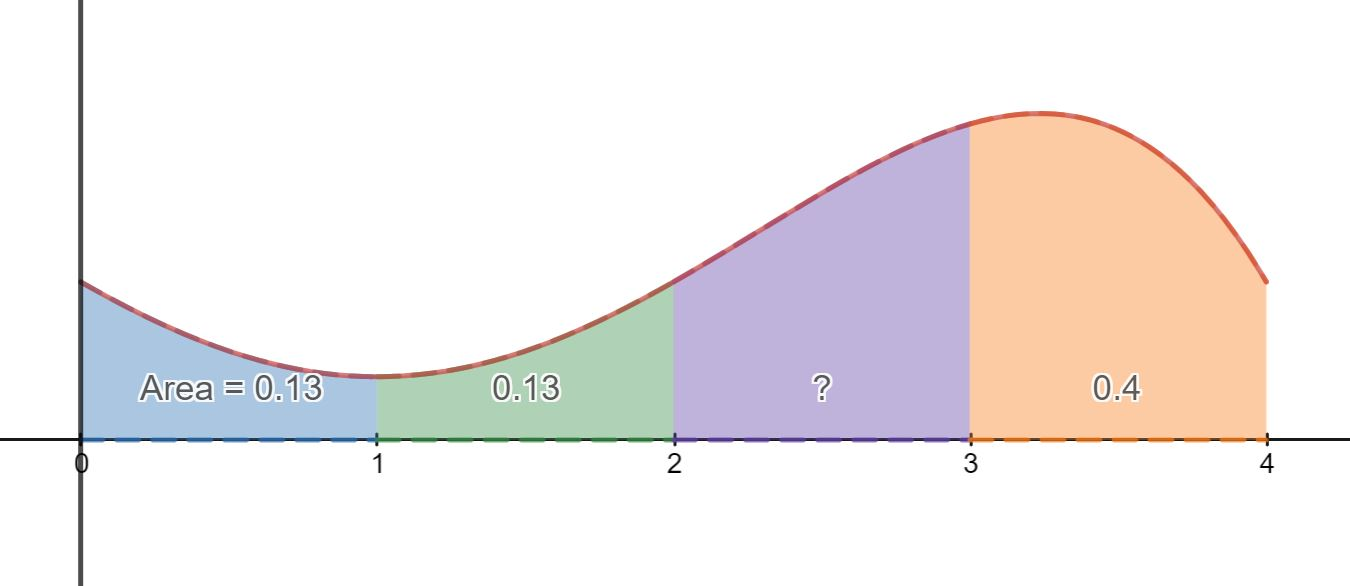
\includegraphics[height=1in]{140H4pic2.jpg}~
 
\end{image}
\begin{enumerate}
    \item Find the missing area.  
    $$A=\answer{0.34}$$
    \item Find each of the following:
    $$P(x=1)=\answer{0}$$
    $$P(1\leq x\leq 2)=\answer{0.13}$$
    $$P(1\leq x\leq 3)=\answer{0.47}$$
    $$P(x>3)=\answer{0.4}$$
    $$P(x=1.5)=\answer{0}$$
    
\end{enumerate}
\end{problem}


\end{document}